\documentclass[../main.tex]{subfiles}
\begin{document}
	
	\chapter{Álgebra Vetorial e Geometria Analítica}
	Para iniciar os estudos de Álgebra Linear, é interessante apresentar, inicialmente, conceitos básicos para visualizar e estruturar o conhecimento. Nesse sentido, entender vetores na perspectiva geométrica, ou seja, no plano ($\mathbb{R}^2$) ou no espaço ($\mathbb{R}^3$), é mais intuitivo em um primeiro contato. Nos próximos capítulos, em especial no capítulo 3, a definição de vetores será ampliada para outros espaços vetoriais, com um maior nível de abstração.
	
	\section{Álgebra Vetorial}
		Embora iniciemos com Álgebra Vetorial e não Geometria Analítica, é interessante começar com um ponto de vista mais geométrico, para criar intuição.
		\begin{definicao}
			\azul{Vetores (geometricamente)} são objetos matemáticos que possuem módulo, direção e sentido.
			
			Usualmente, um vetor é representado por segmentos de retas orientados equipolentes, ou seja, que apresentam mesmo tamanho, direção e sentido.
			\begin{center}
				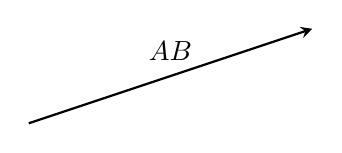
\begin{tikzpicture}[scale=1.2, >=stealth]
					\draw[thick] [->] (0,0) -- (3,1) node[midway, above=2pt] {$\vv{AB}$};
				\end{tikzpicture}
			\end{center}
		\end{definicao}
		Note que, pela definição, um vetor não possui "origem fixa" e pode ser representado por diferentes segmentos de reta orientados.
		\begin{definicao}
			Sejam $U$ e $V$ vetores representados por $\vv{AB}$ e $\vv{BC}$, respectivamente. A \azul{soma de vetores} $U+V$ é definida como o vetor representado pelo segmento de reta orientado $\vv{AC}$  
			\begin{center}
				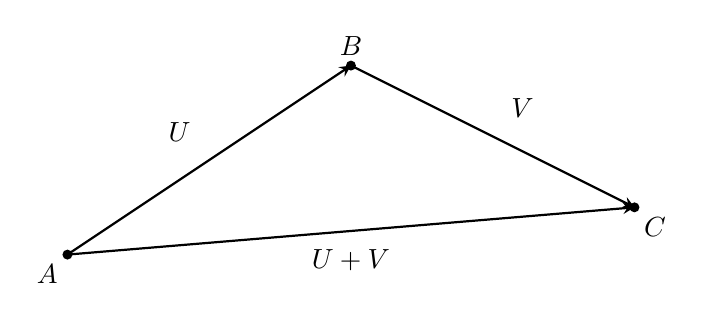
\begin{tikzpicture}[scale=1.2, >=stealth]
					% Pontos
					\coordinate (A) at (0,0);
					\coordinate (B) at (3,2);
					\coordinate (C) at (6,0.5);
					
					% Lados com setas
					\draw[thick, ->] (A) -- (B) node[midway, above left=3pt] {$U$};
					\draw[thick, ->] (B) -- (C) node[midway, above right=3pt] {$V$};
					\draw[thick, ->] (A) -- (C) node[midway, below=3pt] {$U+V$};
					
					% Pontos marcados
					\fill (A) circle (1.5pt) node[below left] {$A$};
					\fill (B) circle (1.5pt) node[above] {$B$};
					\fill (C) circle (1.5pt) node[below right] {$C$};
				\end{tikzpicture}
			\end{center}
		\end{definicao}
		\begin{proposicao}
			Sejam $V$, $W$ e $U$ vetores.
			A soma de vetores segue as seguintes propriedades:
			\begin{enumerate}[label=\roman*)]
				\item $V+W=W+V$ (comutatividade)
				\item $V+(W+U)=(V+W)+U$ (associatividade)
				\item $\exists \text{ vetor }\bar{0}\text{, tal que }  V+\bar{0}=V$ (existência do elemento neutro/vetor nulo)
			\end{enumerate}
		\end{proposicao}
		Abaixo seguem ilustrações das propriedades i) e ii).
		\begin{figure}[h!]
			\centering
			\begin{minipage}{0.45\textwidth}
				\centering
				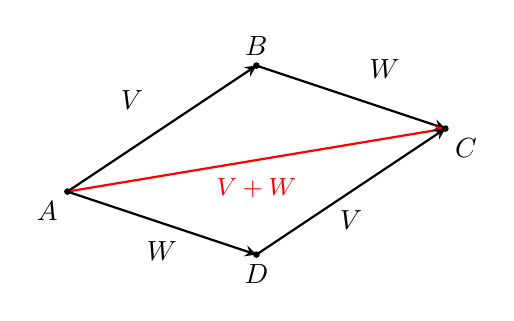
\begin{tikzpicture}[scale=0.8, >=stealth]
					% Pontos
					\coordinate (A) at (0,0);
					\coordinate (B) at (3,2);
					\coordinate (C) at (6,1);
					\coordinate (D) at (3,-1);
					
					% Lados com setas
					\draw[thick, ->] (A) -- (B) node[midway, above left=3pt] {$V$};
					\draw[thick, ->] (B) -- (C) node[midway, above right=3pt] {$W$};
					\draw[thick, ->, red] (A) -- (C) node[midway, below=3pt] {\small $V+W$};
					\draw[thick, ->] (A) -- (D) node[midway, below=3pt] {$W$};
					\draw[thick, ->] (D) -- (C) node[midway, below=3pt] {$V$};
					
					% Pontos marcados
					\fill (A) circle (1.5pt) node[below left] {$A$};
					\fill (B) circle (1.5pt) node[above] {$B$};
					\fill (C) circle (1.5pt) node[below right] {$C$};
					\fill (D) circle (1.5pt) node[below] {$D$};
				\end{tikzpicture}
			\end{minipage}
			\hfill
			\begin{minipage}{0.45\textwidth}
				\centering
				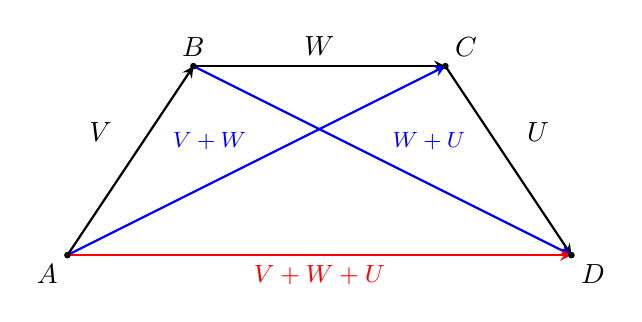
\begin{tikzpicture}[scale=0.8, >=stealth]
					% Pontos
					\coordinate (A) at (0,0);
					\coordinate (B) at (2,3);
					\coordinate (C) at (6,3);
					\coordinate (D) at (8,0);
					
					% Lados com setas
					\draw[thick, ->] (A) -- (B) node[midway, above left=3pt] {$V$};
					\draw[thick, ->] (B) -- (C) node[midway, above] {$W$};
					\draw[thick, ->] (C) -- (D) node[midway, above right=3pt] {$U$};
					\draw[thick, ->, blue] (A) -- (C) node[midway, above left] {\footnotesize $V+W$};
					\draw[thick, ->, blue] (B) -- (D) node[midway, above right] {\footnotesize $W+U$};
					\draw[thick, ->, red] (A) -- (D) node[midway, below] {\small $V+W+U$};
					
					% Pontos marcados
					\fill (A) circle (1.5pt) node[below left] {$A$};
					\fill (B) circle (1.5pt) node[above] {$B$};
					\fill (C) circle (1.5pt) node[above right] {$C$};
					\fill (D) circle (1.5pt) node[below right] {$D$};
				\end{tikzpicture}
			\end{minipage}
		\end{figure}
		\begin{definicao}
			Seja $V$ um vetor. Seu \azul{simétrico}, denotado por $-V$, é o vetor tal que
			\[
			V+(-V)=\bar{0}
			\]
		\end{definicao}
		\begin{definicao}
			Sejam $V$ e $W$ vetores. A \azul{diferença $W$ menos $V$} é definida como
			\[
			W-V=W+(-V)
			\]
		\end{definicao}
		\begin{definicao}
			Sejam $V\neq \bar{0}$ um vetor e $\alpha\neq 0$ um escalar (ou seja, um número real). A \azul{multiplicação do vetor $V$ por um escalar $\alpha$}, denotada por $\alpha V$, é definida pelo vetor tal que:
			\begin{enumerate}[label=\roman*)]
				\item seu módulo é $|\alpha||V|$, onde $|V|$ é o módulo de $V$;
				\item a direção é a mesma de $V$;
				\item tem sentido de $V$ se $\alpha>0$, e sentido de $-V$ se $\alpha<0$.
			\end{enumerate}
			Caso $V=\bar{0}$ ou $\alpha=0$, $\alpha V=\bar{0}$
		\end{definicao}
		\begin{definicao}
			Seja $V$ um vetor. As \azul{componentes de V} são cada elemento das coordenadas que representam o ponto final com relação à origem do sistema de coordenadas escolhido.
			
			Se $V$ está no plano (\azul{$\mathbb{R}^2$} ou \azul{espaço euclidiano bidimensional}), então suas coordenadas são uma trupla de dois números reais, denotadas usualmente por $(v_1, v_2)$.
			
			Se $V$ está no espaço (\azul{$\mathbb{R}^3$} ou \azul{espaço euclidiano tridimensional}), então suas coordenadas são uma tupla de três números reais, denotadas usualmente por $(v_1, v_2, v_3)$.
			
			Se $V$ está em "dimensões maiores" (\azul{$\mathbb{R}^n$} ou \azul{espaço euclidiano n-dimensional}), então suas coordenadas são uma tupla de $n$ números reais, denotadas usualmente por $(v_1, \dots, v_n)$.
		\end{definicao}
		Abaixo seguem ilustrações de como coordenadas funcionam no plano e no espaço.
		\begin{figure}[h]
			\centering
			
			% --- subfigura R^2 ---
			\begin{subfigure}[t]{0.48\textwidth}
				\centering
				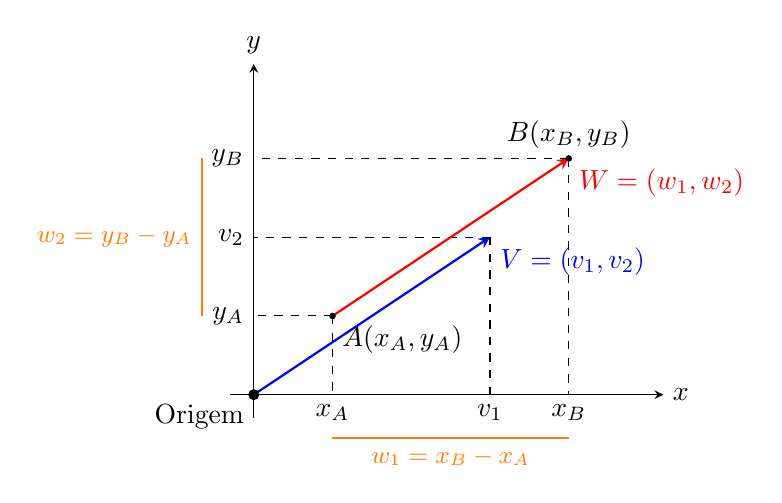
\begin{tikzpicture}[>=stealth,scale=1.0] % pode ajustar a escala se quiser
					% Eixos
					\draw[->] (-0.3,0) -- (5.2,0) node[right] {$x$};
					\draw[->] (0,-0.3) -- (0,4.2) node[above] {$y$};
					
					\coordinate (O) at (0,0);
					\coordinate (P) at (3,2);   % ponto de v
					\coordinate (A) at (1,1);   % ponto inicial de w
					\coordinate (B) at (4,3);   % ponto final de w
					
					% Vetor na origem
					\draw[->,thick,blue] (O) -- (P)
					node[below right] {$V=(v_1,v_2)$};
					
					% Projeções de v
					\draw[dashed] (P) -- (3,0) node[below] {$v_1$};
					\draw[dashed] (P) -- (0,2) node[left] {$v_2$};
					
					% Vetor deslocado
					\draw[->,thick,red] (A) -- (B)
					node[below right] {$W=(w_1,w_2)$};
					
					% Pontos A e B e orgigem
					\fill (A) circle (1.2pt) node[below right] {$A(x_A,y_A)$};
					\fill (B) circle (1.2pt) node[above] {$B(x_B,y_B)$};
					\fill (O) circle (2pt) node[below left] {\text{Origem}};
					
					% Projeções para mostrar diferenças
					\draw[dashed] (A) -- (1,0) node[below] {$x_A$};
					\draw[dashed] (B) -- (4,0) node[below] {$x_B$};
					\draw[dashed] (A) -- (0,1) node[left] {$y_A$};
					\draw[dashed] (B) -- (0,3) node[left] {$y_B$};
					
					% Segmentos representando as diferenças
					\draw[thick,orange,yshift=-10pt]
					(1,-0.2) -- node[below] {\small $w_1 = x_B - x_A$} (4,-0.2);
					
					\draw[thick,orange,xshift=-13pt]
					(-0.2,1) -- node[left] {\small $w_2 = y_B - y_A$} (-0.2,3);
				\end{tikzpicture}
				\caption{Representação no $\mathbb{R}^2$.}
			\end{subfigure}
			\hfill
			% --- subfigura R^3 ---
			\begin{subfigure}[t]{0.48\textwidth}
				\centering
				\tdplotsetmaincoords{70}{120}
				\begin{tikzpicture}[scale=1.6,tdplot_main_coords,>=stealth]
					% Eixos
					\draw[->] (0,0,0) -- (3,0,0) node[below right] {$x$};
					\draw[->] (0,0,0) -- (0,3,0) node[left] {$y$};
					\draw[->] (0,0,0) -- (0,0,3) node[above] {$z$};
					
					% Vetor na origem
					\coordinate (V) at (1,1.4,3);
					\draw[->,thick,blue] (0,0,0) -- (V)
					node[below right] {$V=(v_1,v_2,v_3)$};
					\fill (0,0,0) circle (1.5pt) node[above left] {\text{Origem}};
					\fill (V) circle (1.5pt) node[above left] {};
					
					% Projeções de v
					\coordinate (Vxy) at (1,1.4,0);
					\coordinate (Vx)  at (1,0,0);
					\coordinate (Vy)  at (0,1.4,0);
					\draw[dashed] (V) -- (Vxy);
					\draw[dashed] (Vxy) -- (Vx) node[above left] {$v_1$};
					\draw[dashed] (Vxy) -- (Vy) node[above right] {$v_2$};
					\draw[dashed] (V) -- (0,0,3) node[left] {$v_3$};
					\draw[dashed] (0,0,0) -- (Vxy);
				\end{tikzpicture}
				\caption{Representação no $\mathbb{R}^3$.}
			\end{subfigure}
			
			\caption{Componentes de vetores em $\mathbb{R}^2$ e $\mathbb{R}^3$.}
			\label{fig:vetores-R2-R3}
		\end{figure}
		
		Perceba que, para verificar as componentes de um vetor qualquer $W$ representado por um segmento $\vv{AB}$, basta subtrair as suas coordenadas, de modo que:
		\[
		W = \vv{AB}\Rightarrow
		\begin{cases}
			w_1 = x_B - x_A\\
			w_2 = y_B - y_A
		\end{cases}\Rightarrow
		W = (x_B - x_A,\, y_B - y_A)
		\]
		Para o $\mathbb{R}^3$, a subtração ocorre da mesma forma.
		
		Com isso, note que as operações ficam muito mais fáceis, sem depender sempre do apelo geométrico. Assim, podemos buscar uma nova forma de fazer as operações básicas entre vetores (soma e multiplicação por escalar):
		\begin{proposicao}
			Sejam $V, W\in \mathbb{R}^2$ e $\alpha\in \mathbb{R}$. Então,
			\begin{enumerate}[label = \roman*)]
				\item $V+W = (v_1+w_1,\, v_2+w_2)$
				\item $\alpha V = (\alpha v_1,\, \alpha v_2)$
			\end{enumerate} 
		\end{proposicao}
		Abaixo temos uma ilustração disso.
		\begin{figure}[h]
			\centering
			
			%----------------- (a) Soma de vetores -----------------
			\begin{subfigure}[t]{0.48\textwidth}
				\centering
				\begin{tikzpicture}[>=stealth,scale=1.2]
					
					% Eixos
					\draw[->] (-0.3,0) -- (4.5,0) node[right] {$x$};
					\draw[->] (0,-0.3) -- (0,3.5) node[above] {$y$};
					
					\coordinate (O) at (0,0);
					\coordinate (V) at (2,1.0);   % V = (v1,v2)
					\coordinate (W) at (1.2,1.6); % W = (w1,w2)
					\coordinate (S) at ($(V)+(W)$); % V+W
					
					% Vetores V e W na origem
					\draw[->,thick,blue] (W) -- (S)
					node[below right] {$ V$};
					\draw[->,thick,red]  (O) -- (W)
					node[above left] {$W$};
					
					% Vetor soma
					\draw[->,thick,green!60!black] (O) -- (S)
					node[above right] {$ V+ W$};
					
					% Projeções
					\draw[dashed] (W) -- (1.2, 0) node[below] {$w_1$};
					\draw[dashed] (W) -- (0, 1.6) node[left] {$w_2$};
					\draw[dashed] (S) -- (3.2, 0) node[below] {$w_1+v_1$};
					\draw[dashed] (S) -- (0, 2.6) node[left] {$w_2+v_2$};
					
					% Segmentos representando as diferenças
					\draw[thick,orange,yshift=-10pt]
					(1.2,-0.2) -- node[below] {\small $v_2$} (3.2,-0.2);
					
					\draw[thick,orange,xshift=-13pt]
					(-0.2,1.6) -- node[left] {\small $v_1$} (-0.2,2.4);
					
				\end{tikzpicture}
				\caption{Soma de vetores: $ V+ W=(v_1+w_1,\;v_2+w_2)$.}
			\end{subfigure}
			\hfill
			%----------------- (b) Multiplicação escalar -----------------
			\begin{subfigure}[t]{0.48\textwidth}
				\centering
				\begin{tikzpicture}[>=stealth,scale=1.2]
					
					% Eixos
					\draw[->] (-0.3,0) -- (4.5,0) node[right] {$x$};
					\draw[->] (0,-0.3) -- (0,3.5) node[above] {$y$};
					
					\coordinate (O) at (0,0);
					\coordinate (V) at (1.8,1.1);     % V
					\def\alpha{2}                      % escolha de alpha > 1
					\coordinate (AV) at ({\alpha*1.8},{\alpha*1.1}); % alpha V
					
					% vetor V
					\draw[->,thick,blue] (0,0) -- (1.8,1.1)
					node[below right] {$V = (v_1,v_2)$};
					
					% vetor 2V um pouco acima, para não ficar em cima de V
					\draw[->,thick,red] (0,0.1) -- (3.6,2.3)
					node[above right] {$2V = (2v_1,2v_2)$};
					
				\end{tikzpicture}
				\caption{Multiplicação escalar: $\alpha V=(\alpha v_1,\alpha v_2)$.}
			\end{subfigure}
			
			\caption{Ilustração da soma de vetores e multiplicação escalar em $\mathbb{R}^2$.}
		\end{figure}
		
		Para o $\mathbb{R}^3$, essas operações ocorrem da mesma forma. Generalizando para qualquer dimensão ($\mathbb{R}^n$), temos:
		
		\begin{proposicao}
			Sejam $V, W\in \mathbb{R}^n$ e $\alpha\in \mathbb{R}$. Então,
			\begin{enumerate}[label = \roman*)]
				\item $V+W = (v_1+w_1,\dots, \, v_n+w_n)$
				\item $\alpha V = (\alpha v_1,\dots ,\, \alpha v_n)$
			\end{enumerate} 
		\end{proposicao}
		E se quisermos fazer ambas as operações ao mesmo tempo? Então teremos uma combinação linear!
		\begin{definicao}
			Sejam $V_1, \dots, V_k \in \mathbb{R}^n$ vetores e $\alpha_1,\dots, \alpha_k \in \mathbb{R}$ escalares. Seja $W$ um vetor tal que
			\[
			W = \alpha_1 V_1 + \dots + \alpha_k V_k 
			\]
			Então, $W$ é \azul{combinação linear} de $V_1, \dots, V_k$.
		\end{definicao}
		Abordaremos melhor esse conceito em tópicos mais a frente, como em sistemas lineares.
		
		A partir da definição de coordenadas e da soma/multiplicação de vetores por meio delas, podemos provar as seguintes propriedades:
		\begin{teorema}
			Sejam $U$, $V$ e $W$ vetores e $\alpha$ e $\beta$ escalares. Então:
			\begin{multicols}{2}
				\begin{enumerate}[label=\roman*)]
					\item $U+V=V+U$;
					\item $(U+V)+W=U+(V+W)$;
					\item $U+\bar{0}=U$;
					\item $U+(-U)=\bar{0}$;
					\item $\alpha(\beta U)=(\alpha \beta)U$;
					\item $\alpha(U+V)=\alpha U+\alpha V$;
					\item $(\alpha+\beta)U=\alpha U+\beta U$;
					\item $1U=U$.
				\end{enumerate}
			\end{multicols}
		\end{teorema}
		
		Outra ideia muito importante é saber o módulo do vetor a partir de seus componentes. Para isso, vamos definir o que chamamos de norma euclidiana.
		\begin{definicao}
			Seja $V\in \mathbb{R}^n$. O seu comprimento, também chamado de \azul{norma de $V$} e denotado por $\|V\|$, é dado por
			\[
			\|V\|=\sqrt{v_1^2 +\dots + v_n^2}
			\]
		\end{definicao}
		
		\begin{exemplo}
			Para um vetor  $V\in \mathbb{R}^2$, temos que
			\[
			\|V\| = \sqrt{v_1^2+v_2^2}
			\]
		\end{exemplo}
		\begin{figure}[h]
			\centering
			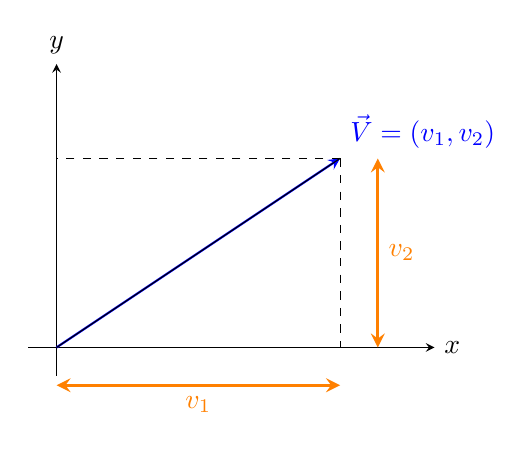
\begin{tikzpicture}[>=stealth,scale=1.2]
				
				% Eixos
				\draw[->] (-0.3,0) -- (4,0) node[right] {$x$};
				\draw[->] (0,-0.3) -- (0,3) node[above] {$y$};
				
				% Vetor V
				\coordinate (O) at (0,0);
				\coordinate (V) at (3,2);   % V = (v1,v2)
				\coordinate (Vx) at (3,0);
				\coordinate (Vy) at (0,2);
				
				\draw[->,thick,blue] (O) -- (V)
				node[above right] {$\vec V=(v_1,v_2)$};
				
				% Projeções para formar o triângulo retângulo
				\draw[dashed] (V) -- (Vx);
				\draw[dashed] (V) -- (Vy);
				
				% Catetos rotulados v1 e v2
				\draw[<->,orange, very thick]
				(0,-0.4) -- node[below] {$v_1$} (3, -0.4);
				\draw[<->,orange,very thick]
				(3.4,0) -- node[right] {$v_2$} (3.4, 2);
				
				% Marcação do ângulo reto
				\tkzMarkRightAngle(V,Vx,O)
				
				% Rótulo da norma na hipotenusa
				\draw (O) -- (V)
				node[midway,above left,yshift=4pt]
				{};
				
			\end{tikzpicture}
			\caption{Norma de um vetor $\vec V$ em $\mathbb{R}^2$.}
		\end{figure}
		Essa forma de calcular a norma está ligada ao cálculo do tamanho de vetores no $\mathbb{R}^2$ e no $\mathbb{R}^3$, utilizando o Teorema de Pitágoras.
		
		A partir dessa definição de norma, podemos definir outro conceito fundamental: o produto escalar. Este produto pega dois vetores e devolve um escalar (número real), que vai indicar o "nível de alinhamento entre eles".
		
		\begin{definicao}
			Sejam $V,\, W\in \mathbb{R}^n$, onde $n\in \{2,3\}$. O \azul{produto escalar} (também conhecido como \azul{produto interno}) entre esses vetores, denotado por $V\cdot W$, é dado por
			\[
			V\cdot W = \begin{cases}
				0\text{, se $V=\bar{0}$ ou $W=\bar{0}$}\\
				\|V\|\|W\|\cos(\theta)\text{, caso contrário.}
			\end{cases}
			\]
			onde $\theta$ é o ângulo no intervalo $[0,\pi]$ entre eles. 
		\end{definicao}
		Note, no entanto, que o ângulo entre dois vetores só é bem definido para vetores em $\mathbb{R}^2$ ou $\mathbb{R}^3$. Para resolver esse problema, podemos encontrar uma definição equivalente para o produto escalar e depois generalizá-la para dimensões maiores.
		\begin{teorema}
			Sejam $V$ e $W$ vetores. Então, seu produto escalar é dado por
			\[
			V\cdot W = \begin{cases}
				v_1w_1+v_2w_2\text{, se $V,W \in \mathbb{R^2}$}\\
					
					v_1 w_1 +v_2 w_2 + v_3 w_3\text{, se $V, W \in \mathbb{R}^3$.}
			\end{cases}
			\]
		\end{teorema}
		A partir disso, podemos definir o produto escalar da seguinte forma generalizada.
		\begin{definicao}
			Sejam $V, W\in \mathbb{R}^n$. O produto escalar entre esses vetores, denotado por $V\cdot W$, é dado por
			\[
			V\cdot W = v_1 w_1+\dots + v_n w_n
			\]
		\end{definicao}
		Com essa definição, podemos facilmente provar as seguintes propriedades (que futuramente definirão de forma ainda mais abrangente o produto interno).
		\begin{teorema}
			Sejam $U,\, V,\, W\in \mathbb{R}^n$ e $\alpha \in \mathbb{R}$. Então:
			\begin{enumerate}[label=\roman*)]
				\item $U\cdot V=V\cdot U$;
				\item $U\cdot (V+W)=U\cdot V+U\cdot W$;
				\item $\alpha(U\cdot V)=(\alpha U)\cdot V = U\cdot (\alpha V)$;
				\item $V\cdot V=\|V\|^2\geq 0,\, \forall V$ e $V\cdot V=0 \Leftrightarrow V = \bar{0}$.
			\end{enumerate}
		\end{teorema}
		As ideias de norma e produto escalar são essenciais e possuem interpretação geométrica. O produto escalar, por exemplo, mostra a relação entre dois vetores e seus tamanhos e "alinhamento" (ângulo entre eles). Isso é muito bem visualizado ao tentarmos entender projeções de um vetor sobre outro: a projeção ortogonal.
		
		\begin{definicao}
			Sejam $V$ e $W$ vetores. A \azul{projeção ortogonal de $V$ sobre $W$}, denotada por $\text{proj}_W V$ é o vetor tal que
			\begin{itemize}
				\item $\text{proj}_W V \parallelsum W$;
				\item $V-\text{proj}_W V \perp W$.
			\end{itemize}
		\end{definicao}
		Abaixo segue uma ilustração da projeção ortogonal.
		\begin{figure}[h]
			\centering
			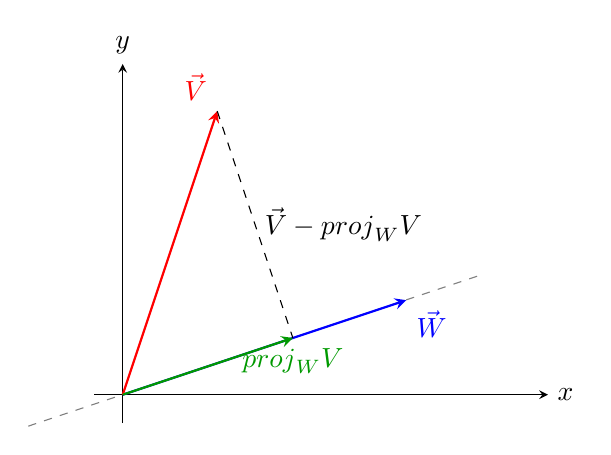
\begin{tikzpicture}[>=stealth,scale=1.2]
				
				% Eixos
				\draw[->] (-0.3,0) -- (4.5,0) node[right] {$x$};
				\draw[->] (0,-0.3) -- (0,3.5) node[above] {$y$};
				
				% Pontos e vetores
				\coordinate (O) at (0,0);
				\coordinate (W) at (3,1);    % direção de W
				\coordinate (V) at (1,3);    % vetor V
				\coordinate (P) at (1.8,0.6);% proj_W V  (ponto na reta de W)
				
				% Reta gerada por W (para ver bem a projeção)
				\draw[dashed,gray] (-1,-1/3) -- (3.8,1.27);
				
				% Vetor W
				\draw[->,thick,blue] (O) -- (W)
				node[below right] {$\vec W$};
				
				% Vetor V
				\draw[->,thick,red] (O) -- (V)
				node[above left] {$\vec V$};
				
				% Projeção de V sobre W
				\draw[->,thick,green!60!black] (O) -- (P)
				node[below] {$\operatorname{proj}_W V$};
				
				% Componente ortogonal V - proj_W V
				\draw[dashed] (V) -- (P)
				node[midway,right] {$\vec V - \operatorname{proj}_W V$};
				
				% Marcação do ângulo reto
				\tkzMarkRightAngle(W,P,V)
				
			\end{tikzpicture}
			\caption{Projeção ortogonal de $\vec V$ sobre $\vec W$.}
		\end{figure}
		A partir dessa definição, podemos provar o seguinte teorema.
		\begin{teorema}
			Seja $W\neq \bar{0}$ um vetor. Então,
			\[
			\text{proj}_W V = \bigg(\frac{V\cdot W}{\|W\|^2}\bigg)W
			\]
		\end{teorema}
		Além do produto escalar, existem outros dois produtos essenciais da Álgebra Vetorial. Enquanto o produto escalar trabalha com "alinhamentos" e projeções, o produto vetorial e misto representam, respectivamente, área e volume.
		\begin{definicao}
			Sejam $V,\, W\in \mathbb{R}^3$. O \azul{produto vetorial} (também conhecido como \azul{produto externo}) entre esses vetores, denotado por $V\times W$, é dado por
			\[
			V\times W = \begin{cases}
				\bar{0}\text{, se $V=\bar{0}$ ou $W=\bar{0}$}\\
				U\text{, caso contrário.}
			\end{cases}
			\]
			onde $U$ é definido como o vetor tal que:
			\begin{enumerate}[label=\roman*)]
				\item $\|U\|=\|V\|\|W\|\sin(\theta)$;
				\item $U\perp V$ e $U\perp W$;
				\item o sentido é dado pela regra da mão direita.
			\end{enumerate}
		\end{definicao}
		A regra da mão direita estabelece que os dedos giram de $V$ para $W$ e o polegar aponta na direção de $U$, representada na Figura \ref{fig:maodireita}.
		
		Utilizando as componentes dos vetores, podemos obter as coordenadas do seu produto vetorial de uma forma mais simples.
		\begin{teorema}
			Sejam $V,\, W\in \mathbb{R}^3$. Então,
			\[
			V\times W = \bigg( \det \begin{bmatrix}
				v_2 & v_3\\
				w_2 & w_3
			\end{bmatrix}, -\det \begin{bmatrix}
				v_1 & v_3\\
				w_1 & w_3
			\end{bmatrix}, \det \begin{bmatrix}
				v_1 & v_2\\
				w_1 & w_2
			\end{bmatrix}\bigg)
			\]
			Ou, utilizando um abuso de notação, temos
			\[
			V\times W = \det \begin{bmatrix}
				\vec i & \vec j & \vec k\\
				v_1 & v_2 & v_3\\
				w_1 & w_2 & w_3
			\end{bmatrix}
			\]
			onde $\vec i=(1, 0, 0)$, $\vec j=(0,1,0)$ e $\vec k=(0,0,1)$ são os \azul{vetores canônicos}.
		\end{teorema}
		\begin{figure}[h]
			\centering
			% vista 3D
			\tdplotsetmaincoords{70}{120}
			\begin{tikzpicture}[tdplot_main_coords,scale=2,>=stealth]
				
				\coordinate (O) at (0,0,0);
				
				% Vetores a e b no plano xy
				\draw[->,thick] (O) -- (2,0,0)
				node[below right] {$V$};
				\draw[->,thick] (O) -- (0,2,0)
				node[below left] {$W$};
				
				% Produto vetorial a x b (polegar)
				\draw[->,very thick,blue] (O) -- (0,0,2)
				node[above] {$V \times W$};
				
				% Arco mostrando o sentido de a para b (sentido dos dedos)
				\draw[->,thick]
				(1.4,0,0) arc[start angle=0,end angle=90,radius=1.4]
				node[midway,below] {$\text{sentido dos dedos}$};
				
			\end{tikzpicture}
			\caption{Regra da mão direita}
			\label{fig:maodireita}
		\end{figure}
		
		Note que, no abuso de notação para representar o produto vetorial, temos que os componentes da matriz são ora vetores, ora números reais, o que indica uma matriz inválida. A ideia dessa representação é de que, se considerássemos $\vec i$, $\vec j$ e $\vec k$ números reais e fizéssemos a conta de tal determinante, e a multiplicação entre reais fosse igual à multipliação por escalar, teríamos o equivalente à primeira forma do produto vetorial, apresentada imediatamente antes. Em suma, essa segunda representação é, na verdade, um "macete" para decorar o produto vetorial.
		
		A partir dessas definições equivalentes do produto vetorial, podemos demonstrar as seguintes propriedades.
		\begin{teorema}
			Sejam $U,\, V,\, W\in \mathbb{R}^3$ e $\alpha \in \mathbb{R}$. Então:
			\begin{enumerate}[label=\roman*)]
				\item $V\times W=-(W\times V)$;
				\item $V\times W=\bar{0}\Leftrightarrow V=\alpha W\text{ ou } W=\alpha V \text{ (ou seja, caso sejam paralelos)}$;
				\item $(V\times W)\cdot V=(V\times W)\cdot W=0$;
				\item $\alpha(V\times W)=(\alpha V)\times W=V\times (\alpha W)$;
				\item $V\times (W+U)=V\times W+V\times U$ e $(V+W)\times U=V\times U+W\times U$.
			\end{enumerate}
		\end{teorema}
		Já o produto misto é dado pela "mistura" dos dois conceitos apresentados anteriormente.
		\begin{definicao}
			Sejam $V,\, W, \, U \in \mathbb{R}^3$. Então, o \azul{produto misto}, denotado por $[V, W, U]$, é dado por
			\[
			[V, W, U]=(V\times W)\cdot U
			\]
		\end{definicao}
		A partir dos conceitos de produto vetorial e escalar, podemos descrever o misto de uma forma facilitada, bem como ressaltar algumas propriedades interessantes.
		\begin{teorema}
			Sejam $V,\, W, \, U \in \mathbb{R}^3$. Então, 
			\[
			[V, W, U]=\det \begin{bmatrix}
				v_1 & v_2 & v_3\\
				w_1 & w_2 & w_3\\
				u_1 & u_2 & u_3
			\end{bmatrix}
			\]
		\end{teorema}
		\begin{teorema}
			Sejam $V,\, W, \, U\in \mathbb{R}^3$ e $\alpha \in \mathbb{R}$. Então,
			\begin{enumerate}[label=\roman*)]
				\item $[U+Z,V,W]=[U,V,W]+[Z,V,W]$
				
				$[U,V+Z,W]=[U,V,W]+[U,Z,W]$
				
				$[U,V,W+Z]=[U,V,W]+[U,V,Z]$;
				\item $[U,V,W]=-[U,W,V]=-[W,V,U]=-[V,U,W]$;
				\item $[U,V,W]=U\cdot(V\times W)$;
				\item $\alpha[U, V, W]=[\alpha U, V, W]=[U, \alpha V, W]=[U, V, \alpha W]$.
			\end{enumerate}
		\end{teorema}
	\section{Geometria Analítica}
	\section{Matrizes como Vetores}
	
\end{document}
